\documentclass[final]{beamer}
\usepackage[numbers]{natbib}
%\usepackage[cm]{fullpage}
%\usepackage[orientation=portrait,size=a0]{beamerposter}
%\usepackage{array,booktabs,tabularx}

\usepackage{float}
\usepackage{grffile}
\mode<presentation>{\usetheme{I6pd2}}
\usepackage[english]{babel}
\usepackage[latin1]{inputenc}
\usepackage{amsmath,amsthm, amssymb, latexsym}
\boldmath
\usepackage[orientation=portrait,size=a1,scale=1.4,debug]{beamerposter}

\usepackage{array,booktabs,tabularx}
\newcolumntype{Z}{>{\centering\arraybackslash}X} % centered tabularx columns
%\newcommand{\pphantom}{\textcolor{ta3aluminium}} % phantom introduces a vertical space in p formatted table columns??!!

\listfiles

\graphicspath{./images/}

\author{Thomas Scarsbrook, Supervisor: Tom Kazmierski}
\title{Ultra-Low Power Logic for Energy Harvesting Systems}
\institute{ECS, Faculty of Physical Sciences and Engineering, University of Southampton, Southampton \\ SO17 1BJ, United Kingdom}
\newcommand{\email}{tos1g09@ecs.soton.ac.uk}
\date{\today}

%\mode<presentation>{
%\usetheme{I6pd2}
%}

%\listfiles

\newcolumntype{Z}{>{\centering\arraybackslash}X} % centered tabularx columns
\newcommand{\pphantom}{\textcolor{ta3aluminium}} % phantom introduces a vertical space in p formatted table columns??!!

\newlength{\columnheight}
\setlength{\columnheight}{70cm}

\begin{document}

\begin{frame}
	\begin{columns}
		\begin{column}{0.49\textwidth}
			\begin{beamercolorbox}[center,wd=\textwidth]{postercolumn}
				\begin{minipage}[T]{0.95\textwidth}
					\parbox[t][\columnheight]{\textwidth}{
						\begin{block}{Introduction}
							Many electronic applications require different system complexities and power usage.
There are two main forms of low power designs, one suited for batteries, one suited for energy harvesting.
\begin{itemize}
	\item Battery
	\begin{itemize}
		\item High power availability
		\item Limited energy
	\end{itemize}
	\item Energy Harvesting
	\begin{itemize}
		\item Low power availability
		\item Theoretically infinite energy
	\end{itemize}
\end{itemize}

Energy harvesting systems often require processing at minimal power expense.
They often run minimalistic tasks, designed to monitor the harvesting system.
Because their source of energy is the same source as is being harvested, the supply can be very small (possibly less than $2\mu W$).
As such, the logic has to operate with minimal draw, as otherwise it will run out of charge and fail, or it will negate the energy source.

There are two main forms of loss in logic circuits, leakage current and switching current.
\\
Leakage current
\begin{itemize}
	\item In transistors current flows between drain and source
	\item Is a small current, but is constant
	\item This is required for correct operation, however current is often larger than it needs to be
\end{itemize}

Switching current
\begin{itemize}
	\item During switching all transistors can be momentarily turned on
	\item Large currents can flow
	\item Energy dumped straight from supply to ground
\end{itemize}

						\end{block}
%						\vfill
						\begin{block}{Sub-Threshold}
							\section{Sub-Threshold Logic}
\label{sec:subthresh}

\subsection{Design}
Sub-threshold logic works by reducing the supply voltage to below the threshold voltage of the transistors.
This uses the leakage current from gate to source as the switching current in the device \cite{ULPSubThresh}.
The main form of current flow in the transistor is the current flowing between the drain and the source.
In subthreshold systems the transistor is in very weak inversion, which means that the channel between the drain and source which is normally open in standard CMOS logic is closed off.
This results in a fraction of the normal current flow than would normally be experienced, this is the `leakage' current.
As the leakage current is exponentially related to the gate voltage, reducing the voltage to below the devices threshold voltage results in the leakage current being greatly reduced.
The knock-on effect of this is an exponential increase in delay can be expected.

The increase in the delay makes subthreshold logic very good for applications which require bursts of computation, spread out over a long period of time.
An example of this can be seen in figure \ref{fig:burstST}.
The upper waveform shows the activity status of a standard CMOS logic gate operating in bursts, when the waveform is at the high level the transistor is active and when the waveform shows low the transistor is inactive.
The lower waveform relates to the activity of a subthreshold circuit.
Under these conditions the standard CMOS logic operates over a time $T$, in this way it rapidly completes the computation and then sits idle, until time $T'$ has passed at which point the computation begins again.
The subthreshold logic, needing longer to complete the calculation, is slowed to take the entiriy of $T'$ to complete.
As such it achieves a large power reduction while providing the same throughput as its standard CMOS equivalent \cite{IEEEVLSIRobustSTL,ULPSubThresh}.

\begin{figure}
	\centering
	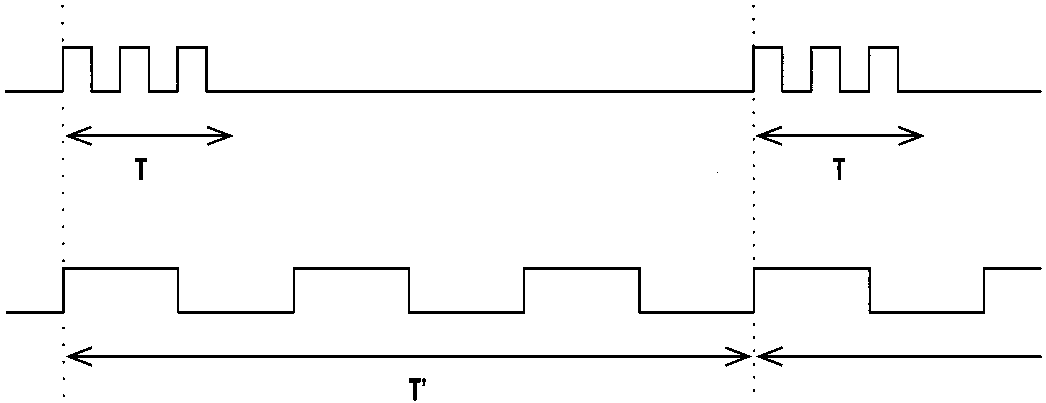
\includegraphics[width=\columnwidth]{../../images/burstycomputation.png}
	\caption{Bursty computation and its relevance to subthreshold operation \cite{IEEEVLSIRobustSTL}}
	\label{fig:burstST}
\end{figure}

In addition to the power saving there are a number of other advantages that subthreshold logic gives.
One of these is an increase in the transconductance gain $gm$ of the device.
Under subthreshold operation the relationship between $V_{gs}$, the voltage across the gate and source, and $I_{ds}$, the current between drain and source, becomes exponential \cite{ULPSubThresh}.
As transconductance gain is defined as $gm = \frac{I_{ds}}{V_{gs}}$, the exponential relationship results in the transconductance gain becoming very large.
Additionally the static noise margin of the device is improved to almost ideal levels.

Furthermore, there are some additional costs in order to achieve the desired power savings.
The devices sensitivity to the temperature, process variations, and power supply noise increases.
As shown in figure \ref{fig:VgsIds} as $V_{gs}$ increases so does the current $I_{ds}$, however the device then enters saturation region at which point $I_{ds}$ levels out.
In this mode of operation, when there is variation on the power supply $V_{gs}$ also varies, however there is minimal change in $I_{ds}$.
With subthreshold logic, the device is operating in the triode region where a change in $V_{gs}$ results in a large change in $I_{ds}$, as such the transconductance gain with respect to the power supply has increased.

\begin{figure}
	\centering
	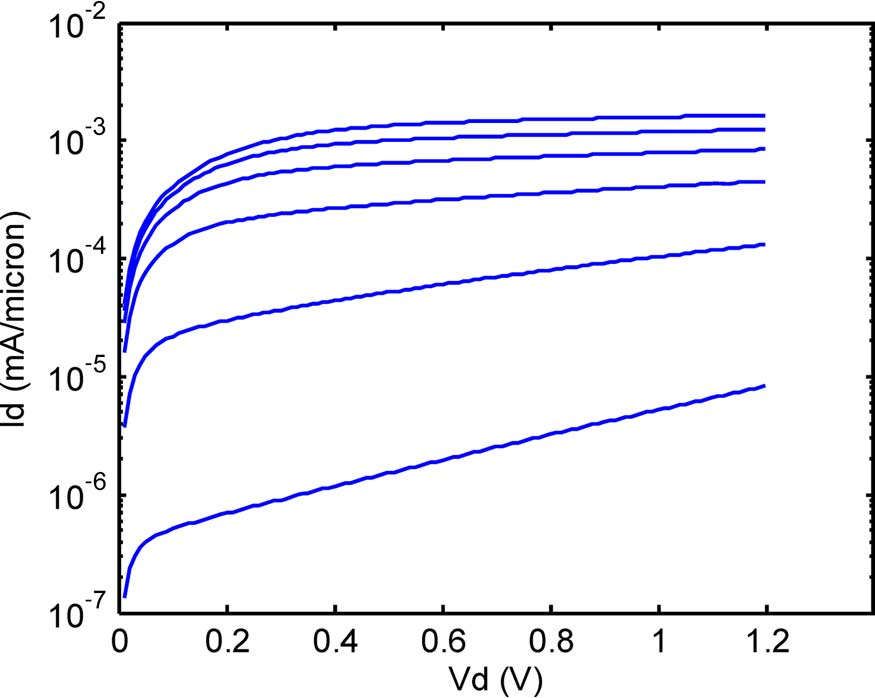
\includegraphics[width=\columnwidth]{../../images/vgsvsids.png}
	\caption{$V_{gs}$ vs. $I_{ds}$ \cite{SemiEmpiricalModels}}
	\label{fig:VgsIds}
\end{figure}

\subsection{Variations}
\subsubsection{Variable Voltage}


\subsubsection{Dynamic Voltage}


						\end{block}
					}
				\end{minipage}
			\end{beamercolorbox}
		\end{column}
		%Change columns
		\begin{column}{0.49\textwidth}
			\begin{beamercolorbox}[center,wd=\textwidth]{postercolumn}
				\begin{minipage}[T]{0.95\textwidth}
					\parbox[t][\columnheight]{\textwidth}{
						\begin{block}{Adiabatic}
							\begin{columns}
	\begin{column}{0.49\textwidth}
		Conventional CMOS logic often has very rapid switching.
		As such the entire supply voltage is briefly across the resistance of the transistors, resulting in a large current flow and large heat dissipation.
	\end{column}
	\begin{column}{0.49\textwidth}
\begin{figure}
	\centering
	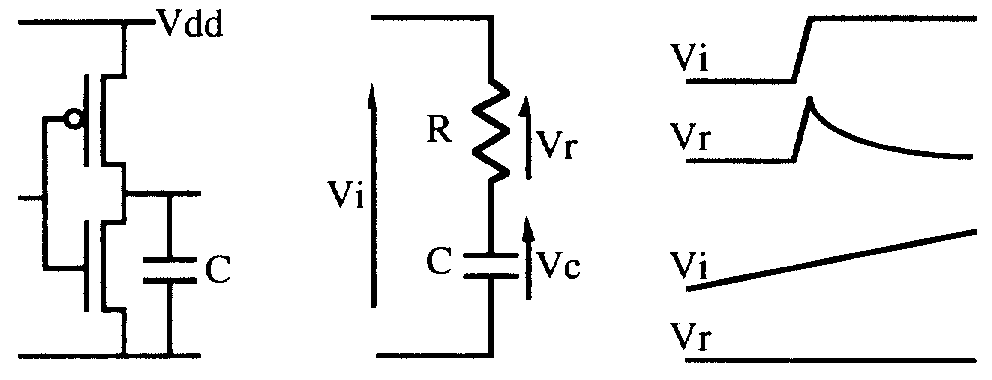
\includegraphics[width=\columnwidth]{../../images/conv_vs_adiabatic.png}
	\caption{Conventional CMOS vs. Adiabatic CMOS in terms of power consumption, shown through the use of the equivalent circuit \cite{DynAdiabatic} }
	\label{fig:convvsadia}
\end{figure}
	\end{column}
\end{columns}

Adiabtic Logic switches much slower, charging up the capacitances with minimal current flow.
There is therefore never a direct short from supply to ground, and heat dissipation is drastically reduced.

In order to achieve the energy saving, adiabatic logic uses a number of stages to set itself up.
Firstly the circuit passes through a \emph{precharge} stage, preloading nodes with a charge.
Then an \emph{evaluation} stage, during which the logical expression is evaluated, and the various nodes either remain charged or discharge as required.
This requirement dictates that adiabatic circuits have a complex clocking circuitry, able to provide two different phases.

\begin{columns}
	\begin{column}{0.49\textwidth}
\begin{figure}
	\centering
	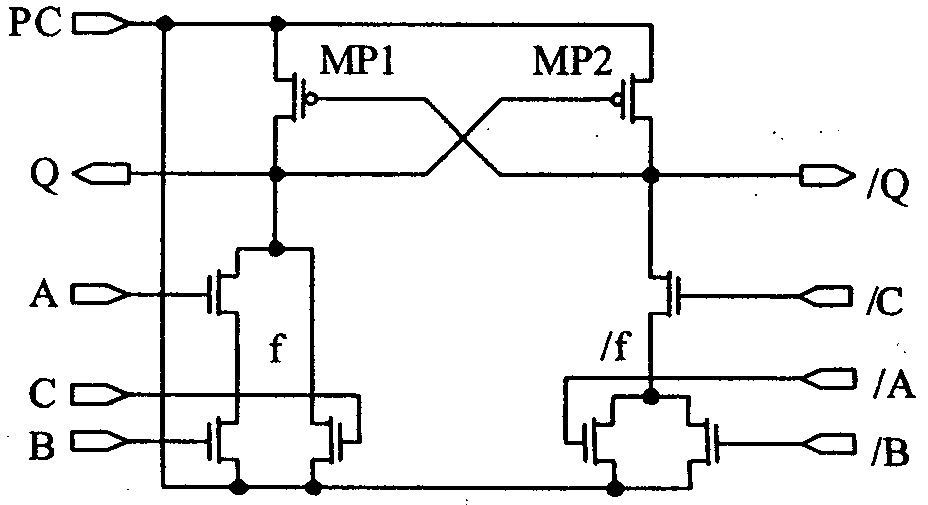
\includegraphics[width=\columnwidth]{../../images/palandor.png}
	\caption{A PAL AND-OR gate ($Q=A.B+C$) showing how to increase the complexity of the circuit \cite{PAL}}
	\label{fig:palandor}
\end{figure}
	\end{column}
	\begin{column}{0.49\textwidth}
		Pass-Transistor Adiabatic Logic (PAL) ia a variation on adiabatic logic requiring only a single clock.
		This clock is sinusoidal, and causes savings of a factor of 10-20.
		Additionally it can provide an inverted output, removing the need for an additional inverter.
	\end{column}
\end{columns}


						\end{block}
%						\vfill
						\begin{block}{Ultra-Low Leakage}
							\section{\acf{ULL}}
\label{sec:ull}

\subsection{notes}

Connect PMOS and NMOS transistors by their sources rather than by their drains.
Biases Vgs negatively, pushing Ioff down to physical limit.


\begin{itemize}

\item Pros:

\begin{itemize}

\item Analogue and digital compatible
\item Simple to design
\item High efficiency
\item Speed relatively unaffected
\item Factor saving in $I_{off}$ of 100-10000 \cite{ULL-AandD}

\end{itemize}

\item Cons:

\begin{itemize}

\item Increases size, each transistor becomes 2 \cite{ULL-AandD}

\end{itemize}

\end{itemize}

\subsection{Design}

Of the two main forms of loss in CMOS logic, switching and leakage currents, \ac{ULL} works to reduce the leakage currents down to the physical limits of the device.

It is often forgotten in CMOS design that there is not only digital circuitry, but also analogue components as well, as these are required to interface with the physical world.
\citeauthor{ULL-AandD} help address this by producing a number of analogue components, as well as digital ones.
Among their designs are voltage followers, transistors, and diodes.

Initially a pair of N and P channel MOSFETs are selected with appropriate $V_{Th}$ values such that their $I_{D}-V_{GS}$ curves intersect at a low current.
These transistors are then connected up in such a way that the P-channel and N-channel transistors are connected by their sources.
This is contradictory to the standard arrangement of transistors, where the transistors would connect via their drains.
The effect of connecting the transistors up this way is that the


\subsection{Variations}


						\end{block}
%						\vfill
						\begin{block}{Conclusion}
							\section{Conclusion}

						\end{block}
					}
				\end{minipage}
			\end{beamercolorbox}
		\end{column}
	\end{columns}
%	\begin{beamercolorbox}[center,wd=\textwidth]{postercolumn}
%		\begin{block}
			\bibliographystyle{IEEEtranN}
			\bibliography{../../sources}
%		\end{block}
%	\end{beamercolorbox}
	\vskip1ex
	\tiny\hfill{Created with \LaTeX \texttt{beamerposter}, template created by Thomas Deselaers and Philippe Dreuw}
\end{frame}

\end{document}
